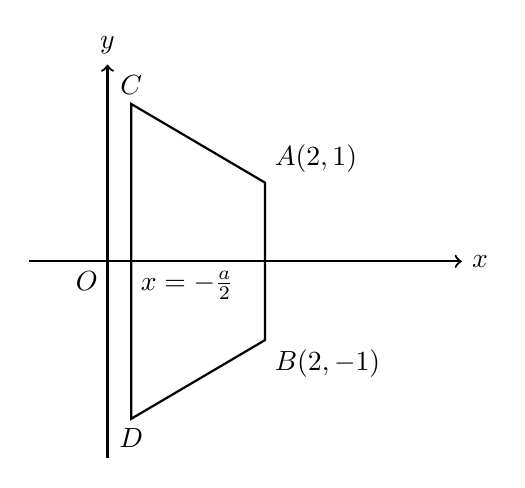
\begin{tikzpicture}[scale=1.0]
    % 绘制坐标轴
    \draw[->, thick] (-1, 0) -- (4.5, 0) node[right] {$x$};
    \draw[->, thick] (0, -2.5) -- (0, 2.5) node[above] {$y$};
    \node[below left] at (0,0) {$O$};

    % 定义点 A, B, C, D 的坐标
    % A(2,1), B(2,-1) 为 z^2-4z+5=0 的两根
    \coordinate (A) at (2, 1);
    \coordinate (B) at (2, -1);
    
    % 当 Delta < 0 时，C 和 D 是一对共轭虚根，实部相同，虚部互为相反数
    % 根据方程 z^2 + az + 9 = 0，由求根公式 z = -a/2 \pm \frac{\sqrt{36-a^2}}{2}i
    % 为了展示 C, D 不在 y 轴上的普遍情况，取 a = -2 作为示意
    % 此时实部 x = -(-2)/2 = 1，虚部 y = \pm \frac{\sqrt{36-4}}{2} = \pm \sqrt{8} \approx \pm 2.83
    % 缩放绘图比例，在图上大致取 (1, 2) 和 (1, -2)
    \coordinate (C) at (0.3, 2);
    \coordinate (D) at (0.3, -2);

    % 绘制等腰梯形 ACDB
    \draw[thick] (A) -- (C) -- (D) -- (B) -- cycle;
    
    % 绘制垂直连线 AB 和 CD
    \draw[dashed, thick] (A) -- (B);
    \draw[dashed, thick] (C) -- (D);

    % 标注 CD 所在的直线方程
    \node[below right] at (0.3, 0) {$x = -\frac{a}{2}$};

    % 标注点
    \node[above right] at (A) {$A(2,1)$};
    \node[below right] at (B) {$B(2,-1)$};
    \node[above ] at (C) {$C$};
    \node[below ] at (D) {$D$};
\end{tikzpicture}